\subsection{Self-Supervision in Videos}
\begin{frame}[allowframebreaks]{Self-Supervision in Videos}
    \begin{itemize}
        \item \textbf{Temporal Order:} Learning to predict or verify the correct temporal sequence of video frames as a self-supervised task.
        \item \textbf{Cycle Consistency:} Enforcing that transformations applied to video frames or clips can be reversed, ensuring consistency in learned representations.
        \item \textbf{Video Speedup:} Training models to recognize or reconstruct videos at different playback speeds, encouraging temporal understanding.
        \item \textbf{Video Colorization:} Using the task of colorizing grayscale video frames as a self-supervised signal for learning spatiotemporal features.
    \end{itemize}
    \begin{figure}
        \centering
        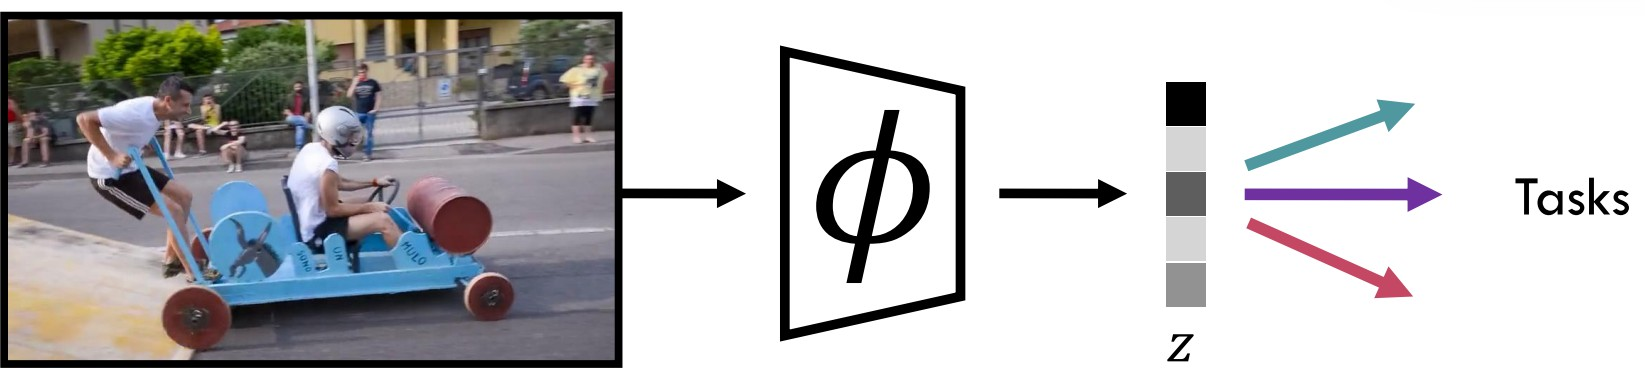
\includegraphics[width=1\textwidth,height=0.25\textheight,keepaspectratio]{images/video/slide_43_1_img.jpg}
    \end{figure}
\end{frame}